\documentclass{article}
\usepackage[utf8]{inputenc}

\title{\textbf{Logic Lab Exercise}}
\author{Laurenz Weixlbaumer\\K11804751\\\texttt{root@fsoc.space}}
\date{November 30, 2021}

% Page dimensions/layout
\usepackage{geometry}

% Images
\usepackage{graphicx}

% Proper quotes
\usepackage{csquotes}

% Proper math
\usepackage{amsmath}
\usepackage{amssymb}

% No indents, par margin
\usepackage{parskip}

% Proper lists
\usepackage{enumitem}

% Listings
\usepackage{listings}

\usepackage{hyperref}

\begin{document}

\begin{titlepage}
\maketitle
\thispagestyle{empty}
\end{titlepage}

Section \ref{sec:analysis} contains an analysis of the evaluation tree for \texttt{testOut2a}(\ldots). The requested screenshots (Figures \ref{fig:correct} and \ref{fig:tree}) as well as a complete listing of the RISCAL file can be found in section \ref{sec:appendix}.

\section{Analysis of the evaluation}
\label{sec:analysis}

We have $a = [2, 0, 1, 3]$, $b = [ 2, 1, 1, 0 ]$, $n = 4$ and $\text{Index} = \mathbb{Z}[-1,5]$.
%
\footnotesize
\begin{equation*}
\begin{split}     
    \text{array}(b, n - 1) \land
    (&\exists\, p: \text{Index.}\ p \geq 0 \land p < n\ \land \\
    (&\forall\, i:\text{Index.}\ (i \geq 0 \land i < n) \Rightarrow (a[p] \leq a[i]))\ \land\\
    (&\forall\, i:\text{Index.}\ (i \geq 0 \land i < p) \Rightarrow (b[i] = a[i]))\ \land\\
    (&\forall\, i:\text{Index.}\ (i \geq 0 \land i < n) \Rightarrow (b[i] = a[i + 1]))
\end{split}
\end{equation*}
\normalsize
%
Let us first consider the outermost conjunction. The left-hand side, $\text{array}(b, n - 1)$, is true since $b$ is an array where all elements at and beyond the index $n - 1 = 3$ are zero. We are left with the existential quantifier on the right-hand side. To evaluate the expression $\exists\, p: \text{Index.}\ F$ we will iteratively apply all possible $p \in \text{Index}$ to $F$.

It will be useful to analyze the trees of subformulas of $\exists$ and $\forall$ in a bottom-up manner --- starting from leaves (or other existential/universal quantifiers, which will themselves be analyzed in this manner) and going toward the root of the subtree.

Thus we have for $p = -1$ (subformula 0 of $\exists$) a leaf of $p \geq 0$ which is false. (In the interest of avoiding redundancy, formulas known to be true or false will be replaced with $\top$ or $\bot$ respectively, instead of being specified manyfold. It will be clear from context what is being replaced.) Going upwards we see that this leads to
\begin{itemize}
    \item $\bot \land (p < n)$ being false, leading to
    \item $\bot \land (\forall\, i:\text{Index.}\ (i \geq 0 \land i < n) \Rightarrow (a[p] \leq a[i]))$ being false, leading to
    \item $\bot \land (\forall\, i:\text{Index.}\ (i \geq 0 \land i < p) \Rightarrow (b[i] = a[i]))$ being false, leading to
    \item $\bot (\forall\, i:\text{Index.}\ (i \geq 0 \land i < n) \Rightarrow (b[i] = a[i + 1]))$ being false,
\end{itemize}
which finally allows us to conclude that $p = -1$ is not the value we seek.

Thus we continue with $p = 0$ (subformula 1 of $\exists$), where, on our way down the tree, we encounter an universal quantifier $\forall\, i:\text{Index.}\ F$. We will iterate over all $i \in \text{Index}$ to evaluate the expression and analyze it in a bottom-up manner, as mentioned previously. The leaves make up the expression $((i \geq 0) \land (i < n)) \Rightarrow (a[p] \leq a[i])$. Since we only care about the right-hand side of an implication when the left-hand side is true we will discard iterations where the left-hand side is false.

Therefore let $i = 1$. Our leaves on the left-hand side are $i \geq 0$ and $i < n$, both of which are true. We then have $\top \land \top$, leading to $\top \Rightarrow (a[p] \leq a[i])$. Recall that $a = [2, 0, 1, 3]$, thus $2 \nleq 0$. We now have $\top \Rightarrow \bot$, which is false.

Thus the universal quantifier is false, which leads to
\begin{itemize}
    \item $\bot \land (p \geq 0 \land p < n)$ being false, leading to
    \item $\bot \land (\forall\, i:\text{Index.}\ (i \geq 0 \land i < p) \Rightarrow (b[i] = a[i]))$ being false, leading to
    \item $\bot \land (\forall\, i:\text{Index.}\ (i \geq 0 \land i < n) \Rightarrow (b[i] = a[i + 1]))$ being false,
\end{itemize}
which finally allows us to conclude that $p = 0$ is not the value we seek.

We continue with $p = 1$ (subformula 2 of $\exists$). Again we encounter an universal quantifier $\forall\, i:\text{Index.}$, the leaves of which make up the expression $((i \geq 0) \land (i < n)) \Rightarrow (b[i] = a[i + 1])$. Let $i = 2$, we now have $i \geq 0$ and $i < n$ leading to $\top \Rightarrow (b[i] = a[i + 1])$. Recall that $b = [ 2, 1, 1, 0 ]$, thus $1 \neq 3$ leading to $\top \Rightarrow \bot$ which is false.

Recall that this universal quantifier is part of a series of conjunctions, thus $p = 1$ is not the value we seek.

We continue with $p = 2$ (subformula 3 of $\exists$). Again we encounter an universal quantifier $\forall\, i:\text{Index.}$, the leaves of which make up the expression $((i \geq 0) \land (i < n)) \Rightarrow (a[p] \leq a[i])$. Let $i = 1$, we now have $i \geq 0$ and $i < n$ leading to $\top \Rightarrow (a[p] \leq a[i])$. Since $1 \nleq 0$ we can conclude that $p = 2$ is not the value we seek.

We continue with $p = 3$ (subformula 4 of $\exists$). Again we encounter an universal quantifier $\forall\, i:\text{Index.}$, the leaves of which make up the expression $((i \geq 0) \land (i < n)) \Rightarrow (a[p] \leq a[i])$. Let $i = 0$, we now have $\top \Rightarrow (a[p] \leq a[i])$. Since $3 \nleq 2$ we can conclude that $p = 3$ is not the value we seek.

We continue with $p_1 = 4$ and $p_2 = 5$ (subformulas 5 and 6 of $\exists$). One of our leaves for both of them is $p < n$. Since $n = 4$ this is false for both $p_1$ and $p_2$. Going upwards we see that this conjunction is part of the series of conjunctions our $\exists$ is made up of, so we can conclude that neither $p = 4$ nor $p = 5$ is the value we seek.

Thus there is no $p$ that satisfies our existential quantifier which overall leads to our formula yielding false for the given inputs.

\pagebreak
\section{Appendix}
\label{sec:appendix}

\begin{figure}[htbp]
  \noindent\makebox[\textwidth]{%
      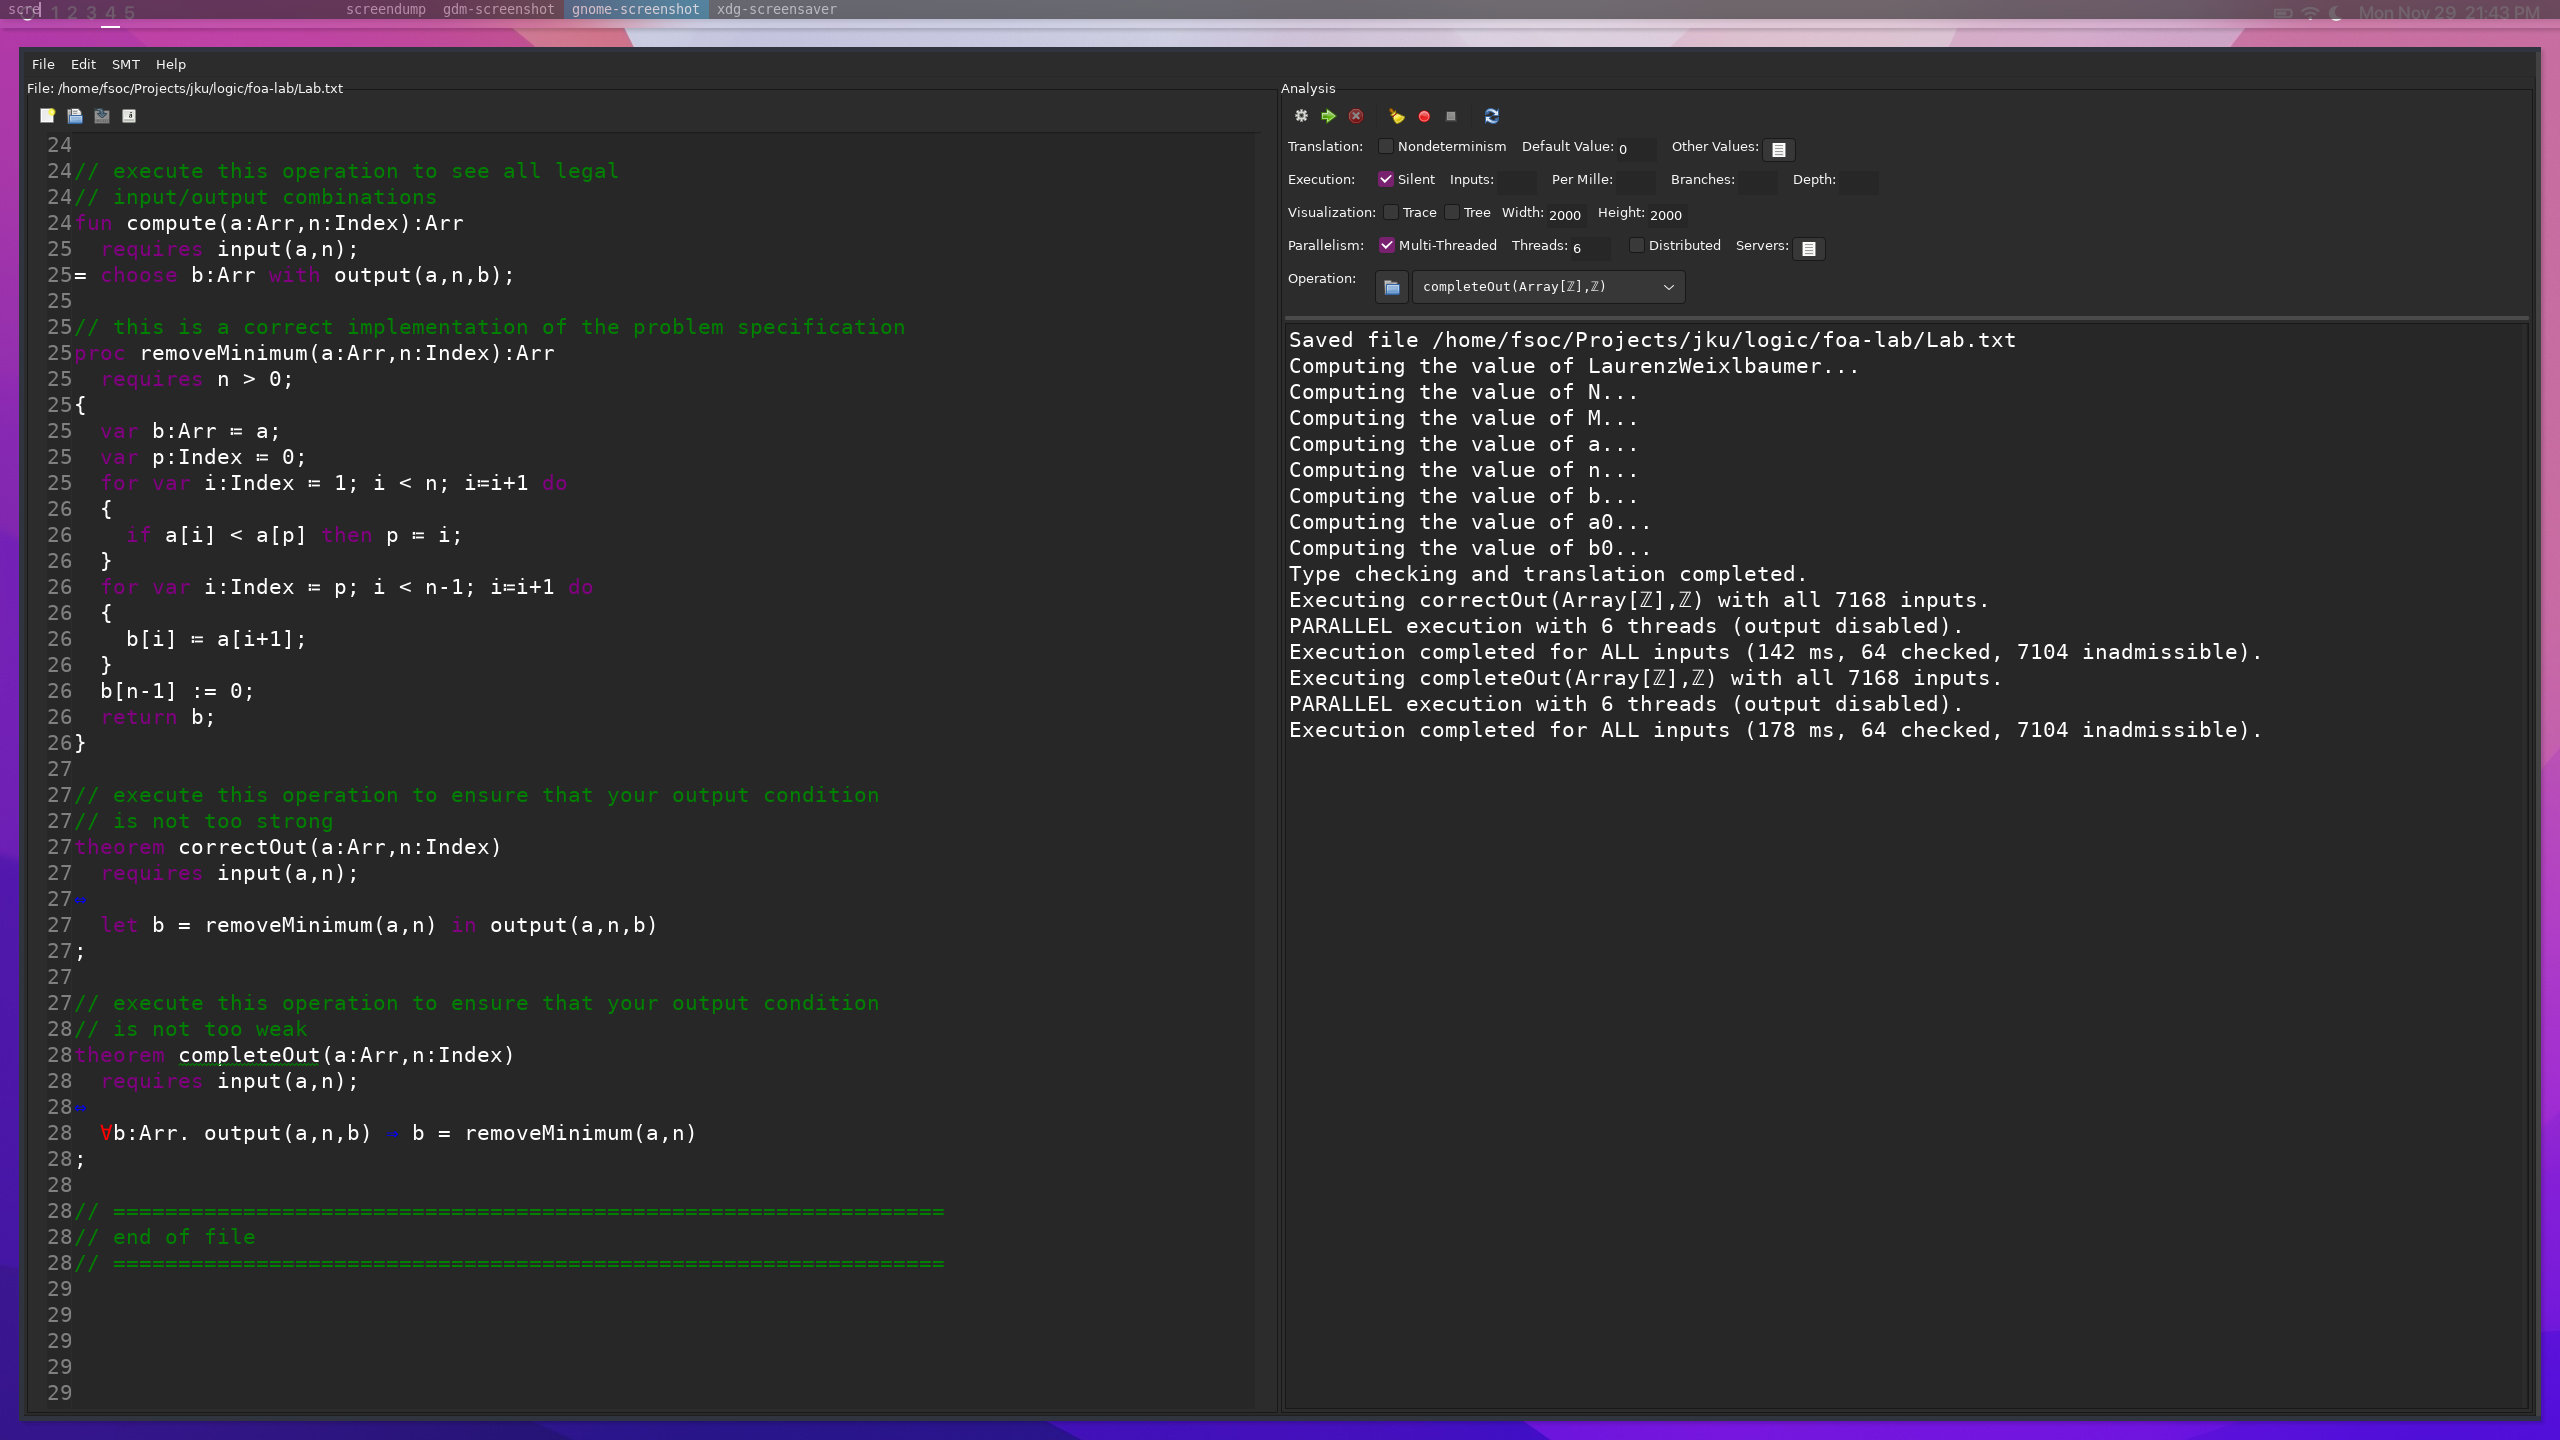
\includegraphics[scale=0.2]{correct.png}
  }

  \caption{Screenshot of the RISCAL terminal output when executing \texttt{correctOut(...)} and \texttt{completeOut(...)}. \label{fig:correct}}
\end{figure}

\begin{figure}[htbp]
  \noindent\makebox[\textwidth]{%
      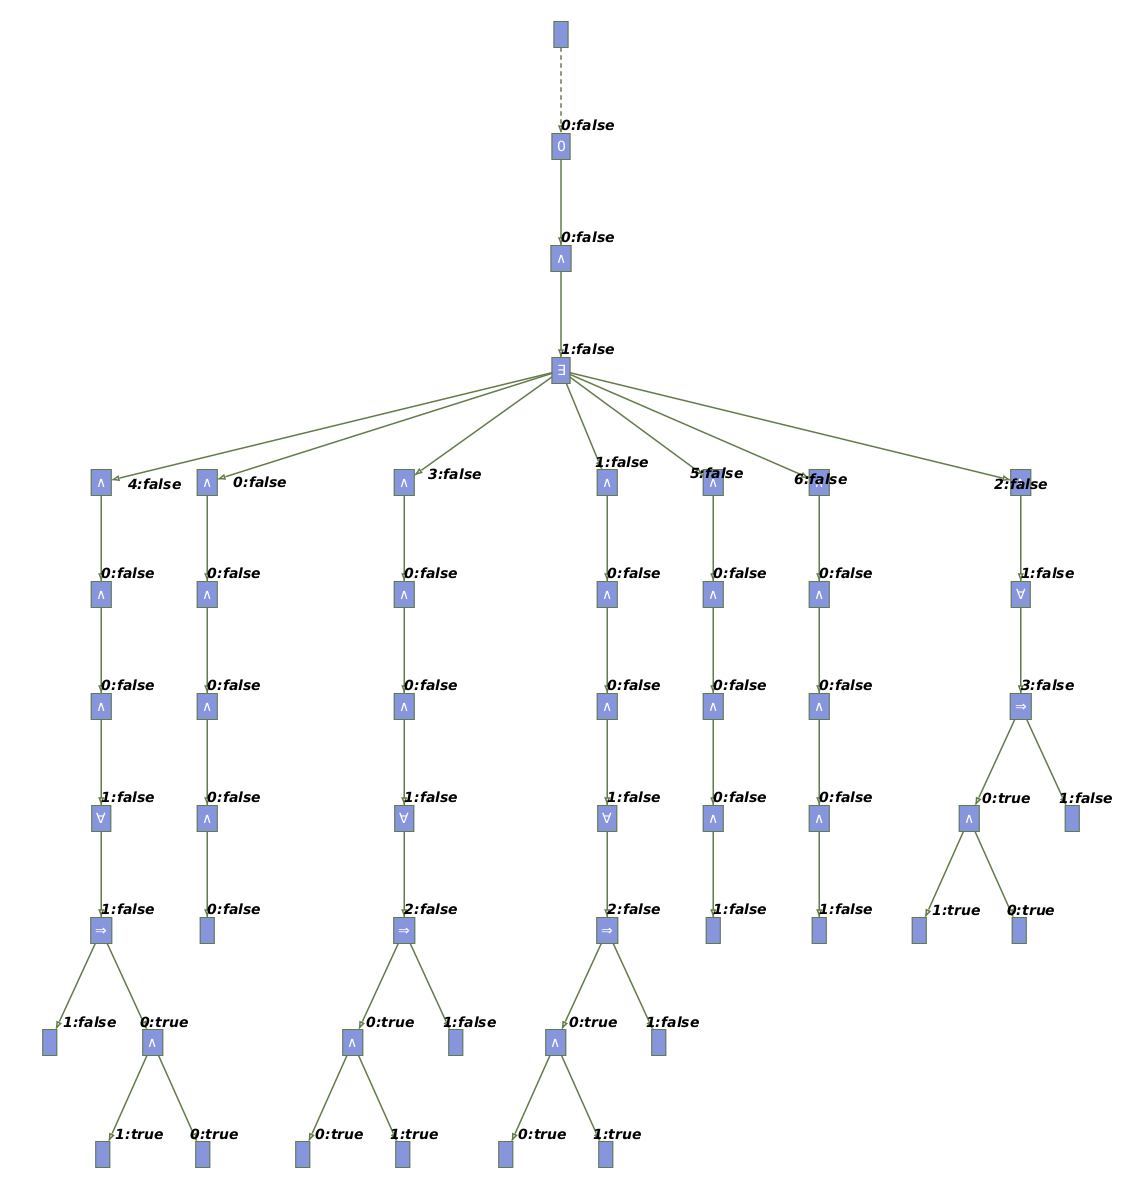
\includegraphics[scale=0.4]{tree-cropped.png}
  }

  \caption{Cropped screenshot of the visualisation tree for \texttt{testOutput2a} (which tests the \texttt{output} predicate) when given an illegal input.  \label{fig:tree}}
\end{figure}

\pagebreak

\begin{lstlisting}[mathescape=true, columns=flexible]
/* ================================================================
   Course Logic, Lab Exercise 
   "Syntax, Semantics, and Pragmatics of First-Order Logic"
   ================================================================
 
 PROBLEM:
 
 Let Elem be the set of all integers in the range 0..M (for some 
 constant M) which we call "elements". Let Arr be the set of all
 "arrays" of length N (for some constant N) of "element" values.
 Let Index be the set of all integers in the range -1..N (which
 includes all valid array indices 0..N-1 but also -1 and N).
 
 We introduce the predicate "a has n elements" to state that the
 last N-n slots a[n],..,a[N-1] of array "a" are filled with value 0 
 (thus array "a" may have arbitrary elements only in the first "n" 
 slots a[0],..,a[n-1]).
 
 We introduce the predicate "a has no duplicates in the first
 n positions" to state that there are not any two different 
 array indices less than "n" such that "a" holds the same 
 element at those indices.
 
 Now consider the following problem: given an array "a" with n>0
 elements that has no duplicates in the first "n" positions, remove 
 from "a" the smallest element; this results in an array that has 
 n-1 elements. For example, for N=5 and M=3, the legal inputs 
 a=[2,0,1,3,0] and n=4 result in the output b=[2,1,3,0,0].
 Since "a" has no duplicates in the first "n" positions, 
 "b" is uniquely determined.
 
 In more detail, this problem can be described as follows:
 
   Input: a $\in$ Arr, n $\in$ Index where
     n is greater than 0 
     a has n elements
     a has no duplicates in the first n positions
   Output: b $\in$ Arr where
     b has n-1 elements
     there exists some position p $\in$ Index such that
       p is greater equal 0 and less than n
       a[p] is less than equal a[0],...,a[n-1]
       b holds at positions 0,..,p-1  the same values as a
       b holds at positions p,..,n-2 those values that 
          a holds at positions p+1,..,n-1
 
 YOUR TASKS: 
 
 0. Replace the name of the constant "WolfgangSchreiner" given
    below by your own name.
 
 1. Complete the definition of predicate "array(a,n)" below to
    state "a has n elements" (as described above).
 
    Complete the definition of predicate "nodup(a,n)" below to
    state "a has no duplicates in the first n positions" 
    (as described above).
 
    Validate your definitions by executing operations "array(..)"
    and "nodup(...)" with execution option "Silent" *not* selected. 
    This prints the truth values of the predicates for *all* 
    possible inputs. Check that the truth values are as expected.
 
 2. Complete the definition of predicate "input(a,n)" below to
    state the input condition of the problem (as described above).
 
    Validate your input condition by executing the operations
    "testIn1()" and "testIn2()". These check the input condition
    for one legal input and for one illegal input (the first should
    run without error, the second with an error message).
 
 3. Complete the definition of predicate "output(a,n,b)" below to
    state the output condition of the problem (as described above).
 
    Validate your output condition by executing the operations
    "testOut1()" and "testOut2()". These check the output condition
    for one legal output and for one illegal output (the first should
    run without error, the second with an error message).
 
 4. Further validate your input/output conditions by executing 
    "compute(..)" with execution option "Silent" *not* selected
    and translation option "Nondeterminism" selected. This prints 
    all input/output pairs allowed by your specification.
    Check that these pairs conform to your expectations.
 
 5. Finally verify your specification by executing the operations 
    "correctOut()" and "completeOut()".
 
    - If "correctOut()" fails, then your output condition is 
      too strong (or your input condition is too weak).
 
    - If "completeOut()" fails, then your output condition is 
      too weak.
 
    If these checks do not fail, your specification is correct
    (unless your input condition is too strong, which can be
    not ruled out by automatic verification).
 
 DELIVERABLES:
 
 The result of this assignment consists of a document that includes
 the following elements:
 
 1. A complete listing of this file (with your formulas nicely
    formatted and indented).
 
 2. A screenshot of the software displaying in the right terminal
 
    - the text "Computing the value of WolfgangSchreiner..." 
      (where the name "WolfgangSchreiner" is replaced by your name).
 
    - the execution of operations correctOut(..) and completeOut(..) 
      (with execution option "Silent" selected).
 
    For this clear the terminal by pressing the "Clear Output" button
    abeled by a broom, modify and save the file (which results in the
    "Computing..." output) and then run the two operations.
 
 3. A screenshot of the visualization window for operation testOut2a()
    which displays the evaluation of the formula "output()" on an 
    *illegal* output (yielding the truth value "false"). Make sure
 
    - you have inlined the definition of "output" into this operation
      (i.e., do not call "output" but insert its definition)
 
    - you have switched on the visualization option "Tree" (and
      set "Width" to a suitably large value e.g. 800).
 
 4. A systematic and detailed written analysis of the evaluation tree
    for testOut2a() where you describe in detail how the evaluation 
    of each subformula yields the truth value "false" of
    the overall formula.
 
    Please note that the label "n:t" at each arrow denotes the 
    number "n" of the subformula to which the arrow points and 
    its truth value "t"; numbering starts with 0, so the first 
    subformula is the one with label n=0 (subformulas may be
    shuffled by the automatic layout of the graph).
 
    Important: hover with the mouse pointer over each node to see 
    the values of the variables on which each subformula depends and 
    the truth value of the subformula. Use this information
    to explain the overall result.
 
    Take a look at the RISCAL manual, Section 2.9 "Visualizing
    Evaluation Trees", for more details on how to interpret the tree.
 
 You will be asked in your presentation to illustrate points 3 and 4 
 (a laptop will be provided that runs RISCAL with your specification).
 
 */
 
 // ================================================================
 // perform here your changes
 // ================================================================
 
 // replace the name of this constant by your name
 val LaurenzWeixlbaumer = 1 ;
 
 val N = 5; 
 val M = 3;
 
 type Elem = $\mathbb{N}$[M];
 type Index = $\mathbb{Z}$[-1,N];
 type Arr = Array[N,Elem];
 
 pred array(a:Arr,n:Index) 
   requires n $\geq$ 0;
 $\Leftrightarrow$
   // formulate here "a has n elements"
   $\forall$i:Index. ((i $\geq$ n $\land$ i < N) $\Rightarrow$ (a[i] = 0))
 ;
 
 pred nodup(a:Arr,n:Index) 
   requires n $\geq$ 0;
 $\Leftrightarrow$
   // formulate here "a has no duplicates in the first n positions"
   $\forall$i:Index. ((i $\geq$ 0 $\land$ i < n) $\Rightarrow$ (
     $\forall$j:Index. (j $\geq$ 0 $\land$ j < i) $\Rightarrow$ (a[j] $\neq$ a[i]))
   )
 ;
 
 pred input(a:Arr,n:Index) $\Leftrightarrow$
   // formulate here the input condition
   n > 0 $\land$ array(a, n) $\land$ nodup(a, n)
 ;
 
 pred output(a:Arr,n:Index,b:Arr) 
   requires n > 0;
 $\Leftrightarrow$
   // formulate here the output condition
   array(b, n - 1) $\land$
   ($\exists$p:Index. p $\geq$ 0 $\land$ p < n $\land$ (
     $\forall$i:Index. (i $\geq$ 0 $\land$ i < n) $\Rightarrow$ (a[p] $\leq$ a[i])
   ) $\land$ (
     $\forall$i:Index. (i $\geq$ 0 $\land$ i < p) $\Rightarrow$ (b[i] = a[i])
   ) $\land$ (
     $\forall$i:Index. (i $\geq$ p $\land$ i < n - 1) $\Rightarrow$ (b[i] = a[i + 1])
   ))
 ;
 
 // ================================================================
 // no more changes needed below (except for testOut2a())
 // ================================================================
 
 // legal inputs a,n and output b
 val a = Array[N,Elem](0) 
   with [0]=2 with [1]=0 with [2]=1 with [3]=3;
 val n = 4 ;
 val b = Array[N,Elem](0) 
   with [0]=2 with [1]=1 with [2]=3;
   
 // illegal input a0 and illegal output b0
 val a0 = Array[N,Elem](0) 
   with [0]=2 with [1]=3 with [2]=1 with [3]=3;
 val b0 = Array[N,Elem](0) 
   with [0]=2 with [1]=1 with [2]=1;
 
 // execute this operation to ensure that your input condition
 // holds/does not hold for the sample inputs
 theorem testIn1() $\Leftrightarrow$ input(a,n);
 theorem testIn2() $\Leftrightarrow$ let a = a0 in input(a,n);
 
 // execute this operation to ensure that your output condition
 // holds for the sample inputs and the correct output
 theorem testOut1() $\Leftrightarrow$ output(a,n,b);
 
 // execute this operation to ensure that your output condition
 // does *not* hold for the sample inputs and a *wrong* output
 theorem testOut2() $\Leftrightarrow$ let b = b0 in output(a,n,b);
 
 // the visualization gets nicer if you inline the postcondition
 // formula and then run this operation
 theorem testOut2a() $\Leftrightarrow$
   let b = b0 in
   // inline here your postcondition formula  
   array(b, n - 1) $\land$
   ($\exists$p:Index. p $\geq$ 0 $\land$ p < n $\land$ (
     $\forall$i:Index. (i $\geq$ 0 $\land$ i < n) $\Rightarrow$ (a[p] $\leq$ a[i])
   ) $\land$ (
     $\forall$i:Index. (i $\geq$ 0 $\land$ i < p) $\Rightarrow$ (b[i] = a[i])
   ) $\land$ (
     $\forall$i:Index. (i $\geq$ p $\land$ i < n - 1) $\Rightarrow$ (b[i] = a[i + 1])
   ))
 ;
 
 // execute this operation to see all legal
 // input/output combinations
 fun compute(a:Arr,n:Index):Arr
   requires input(a,n);
 = choose b:Arr with output(a,n,b);
 
 // this is a correct implementation of the problem specification
 proc removeMinimum(a:Arr,n:Index):Arr
   requires n > 0;
 {
   var b:Arr := a;
   var p:Index := 0;
   for var i:Index := 1; i < n; i:=i+1 do
   {
     if a[i] < a[p] then p := i;
   }
   for var i:Index := p; i < n-1; i:=i+1 do
   {
     b[i] := a[i+1];
   }
   b[n-1] := 0;
   return b;
 }
 
 // execute this operation to ensure that your output condition
 // is not too strong
 theorem correctOut(a:Arr,n:Index) 
   requires input(a,n);
 $\Leftrightarrow$
   let b = removeMinimum(a,n) in output(a,n,b)
 ;
 
 // execute this operation to ensure that your output condition
 // is not too weak
 theorem completeOut(a:Arr,n:Index) 
   requires input(a,n);
 $\Leftrightarrow$
   $\forall$b:Arr. output(a,n,b) $\Rightarrow$ b = removeMinimum(a,n)
 ;
 
 // ================================================================
 // end of file
 // ================================================================ 
\end{lstlisting}

\end{document}